\chapter{Distribuição do Atendimento}
\label{cap:distribuicao}

\lettrine{N}{este} capítulo, será feito um comentário sobre como o atendimento das creches se distribui pela cidade. Para auxiliar no entendimento, serão exibidos mapas que mostram os dados comentados.

\section{Dados absolutos}

Os mapas na \autoref{ev:mat} apresentam o número de matrículas na cidade em dois períodos diferentes.

\begin{figure}[H]
	\centering
	\includegraphics[width=0.49\linewidth]{../Analises/mapas/MAT_CRECHE_jun-06}
	\includegraphics[width=0.49\linewidth]{../Analises/mapas/MAT_CRECHE_dez-17}
	\caption{Mapas que mostram, em junho de 2006 e dezembro de 2017, respectivamente, a distribuição das matrículas no município.}
	\label{ev:mat}
\end{figure}

A escala utilizada para esses dois mapas foi a mesma. Ela consiste em deixar o maior valor com a cor amarela e o menor com um tom escuro de roxo. Como já se sabe, o número de matrículas aumentou em 95 distritos. O maior valor era de 2555 vagas no Grajaú, em junho de 2006 e passou a ser 12486 em dezembro de 2017, ainda no mesmo distrito.

Com esses dois mapas, uma outra informação aparece. É possível observar que a maior parte das matrículas se concentra nos mesmos lugares. São três os "cinturões das vagas": 

\begin{itemize}
	\item \textit{\textbf{Cinturão Sul:}} Composto por distritos como Grajaú, Capão Redondo, Jardim Ângela e Jardim São Luís.
	\item \textit{\textbf{Cinturão Norte:}} Composto por distritos como Anhanguera, Jaraguá e Brasilândia.
	\item \textit{\textbf{Cinturão Leste:}} Composto por distritos como Itaim Paulista, Lajeado e Cidade Tiradentes.
\end{itemize}

Uma figura animada com a evolução do número de matrículas por trimestre entre junho de 2006 e dezembro de 2017 pode ser vista \href{https://lsflp.github.io/MAC0213/multimidia/MAT_CRECHE.gif}{aqui}.

Os mapas na \autoref{ev:dem} apresentam o tamanho da fila na cidade em três períodos diferentes.

\begin{figure}[H]
	\centering
	\includegraphics[width=0.32\linewidth]{../Analises/mapas/DEM_CRECHE_jun-06}
	\includegraphics[width=0.32\linewidth]{../Analises/mapas/DEM_CRECHE_dez-06}
	\includegraphics[width=0.32\linewidth]{../Analises/mapas/DEM_CRECHE_dez-17}
	\caption{Mapas que mostram, em junho de 2006, dezembro de 2006 e dezembro de 2017, respectivamente, a distribuição da demanda no município.}
	\label{ev:dem}
\end{figure}

A escala dos três mapas tem o mesmo funcionamento dos mapas exibidos anteriormente. Os três mapas foram colocados aqui por causa da sazonalidade da fila, então pode ser feita tanto uma comparação entre o primeiro dado e o último quanto uma comparação entre o mesmo mês em anos diferentes.

Em ambas as comparações, vê-se que a fila, em geral, diminuiu. O maior valor era do distrito Grajaú (3914 crianças na fila), em junho de 2006. Em dezembro de 2006, essa posição era do distrito Jardim São Luís (5671 crianças na fila). Em dezembro de 2017, o distrito Capão Redondo era o campeão (2776 crianças na fila). Com 11 anos e meio de diferença, o tamanho da demanda do primeiro colocado caiu pela metade.

Pode-se observar que a demanda se concentra principalmente no Cinturão Sul, definido acima. São distritos dessa região que lideram o \textit{ranking} da fila, como exibido no \autoref{cap:rankings}. Existe um certo destaque para os Cinturões Norte e Leste, claramente ofuscados pelo Cinturão Sul.

Uma figura animada com a evolução do tamanho da demanda por trimestre entre junho de 2006 e dezembro de 2017 pode ser vista \href{https://lsflp.github.io/MAC0213/multimidia/DEM_CRECHE.gif}{aqui}.

\section{Dados proporcionais}

Na \autoref{ev:matprop}, são exibidos mapas que mostram o quanto cada distrito atende, com creches, a população estimada de 0 a 3 anos.

\begin{figure}[H]
	\centering
	\includegraphics[width=0.49\linewidth]{../Analises/mapas/ATEND_REL_jun-06}
	\includegraphics[width=0.49\linewidth]{../Analises/mapas/ATEND_REL_dez-17}
	\caption{Mapas que mostram, em junho de 2006, e dezembro de 2017, respectivamente, a distribuição das matrículas proporcionais à população, no município.}
	\label{ev:matprop}
\end{figure}

Esses mapas mostram que o atendimento proporcional à população aumentou em quase todos os distritos, menos na República, o único a ter uma diminuição no número de vagas. Mesmo a escala sendo alterada, é possível observar que a maior parte dos distritos fica nas taxas de atendimento entre 0.4 e 0.6 (números que representam 40\% e 60\% da população).

O distrito que liderava esse atendimento proporcional em junho de 2006 era a Barra Funda, com 38.33\% da faixa etária em creches municipais. Em dezembro de 2017, essa posição foi tomada por Marsilac, que atende mais de 100\% da população estimada de 0 a 3 anos. 

Uma figura animada com a evolução do número de matrículas relativas à população por trimestre entre junho de 2006 e dezembro de 2017 pode ser vista \href{https://lsflp.github.io/MAC0213/multimidia/ATEND_REL.gif}{aqui}.

Na \autoref{ev:demprop}, são exibidos mapas que mostram o quanto cada distrito tem de demanda proporcional à população estimada de 0 a 3 anos. Assim como na parte dos dados absolutos, são exibidos três mapas, pelos mesmos motivos. 

Pode-se ver, pela escala da legenda, que essa medida diminuiu na cidade como um todo. É possível observar que os distritos mais centrais possuem seus números sobre maior controle (zonas mais escuras). Marsilac, já conhecido por ser um \textit{outlier}, se destaca nessa figura, por ter uma das menores filas relativas no ano de 2006 e a maior fila relativa em dezembro de 2017.

\begin{figure}[H]
	\centering
	\includegraphics[width=0.32\linewidth]{../Analises/mapas/FILA_REL_jun-06}
	\includegraphics[width=0.32\linewidth]{../Analises/mapas/FILA_REL_dez-06}
	\includegraphics[width=0.32\linewidth]{../Analises/mapas/FILA_REL_dez-17}
	\caption{Mapas que mostram, em junho de 2006, dezembro de 2006 e dezembro de 2017, respectivamente, a distribuição da demanda proporcional à população, no município.}
	\label{ev:demprop}
\end{figure}

Uma figura animada com a evolução do tamanho da demanda relativa à população por trimestre entre junho de 2006 e dezembro de 2017 pode ser vista \href{https://lsflp.github.io/MAC0213/multimidia/FILA_REL.gif}{aqui}.

Nos gráficos de dispersão da \autoref{graf:geral}, também pode-se ver como os distritos evoluíram, entre dezembro de 2006 e dezembro de 2017. Seus eixos são matrículas proporcionais por demanda proporcional. Cada ponto roxo no gráfico representa um distrito.

Observa-se uma mudança no padrão dos distritos, antes concentrados na parte de baixo atendimento relativo, se concentram na parte de baixa demanda, nos dados mais recentes.

\begin{figure}[H]
	\centering
	\includegraphics[width=0.5\linewidth]{../Analises/graficos/agrupamentos/mat_dem_dez-06}
	\includegraphics[width=0.5\linewidth]{../Analises/graficos/agrupamentos/mat_dem_dez-17}
	\caption{Gráficos de dispersão usados para encontrar padrões sobre os distritos.}
	\label{graf:geral}
\end{figure}

\section{Evolução geral}

Os dois mapas na \autoref{ev:geral} confirmam o que já tem sido escrito nesse capítulo e no anterior. Pode-se ver que a maioria dos distritos teve aumento no número de matrículas e queda no tamanho da fila.

Um fato a se notar é que os três cinturões (Sul, Norte e Leste) concentram muito do aumento e muito da queda supracitadas.

\begin{figure}[H]
	\centering
	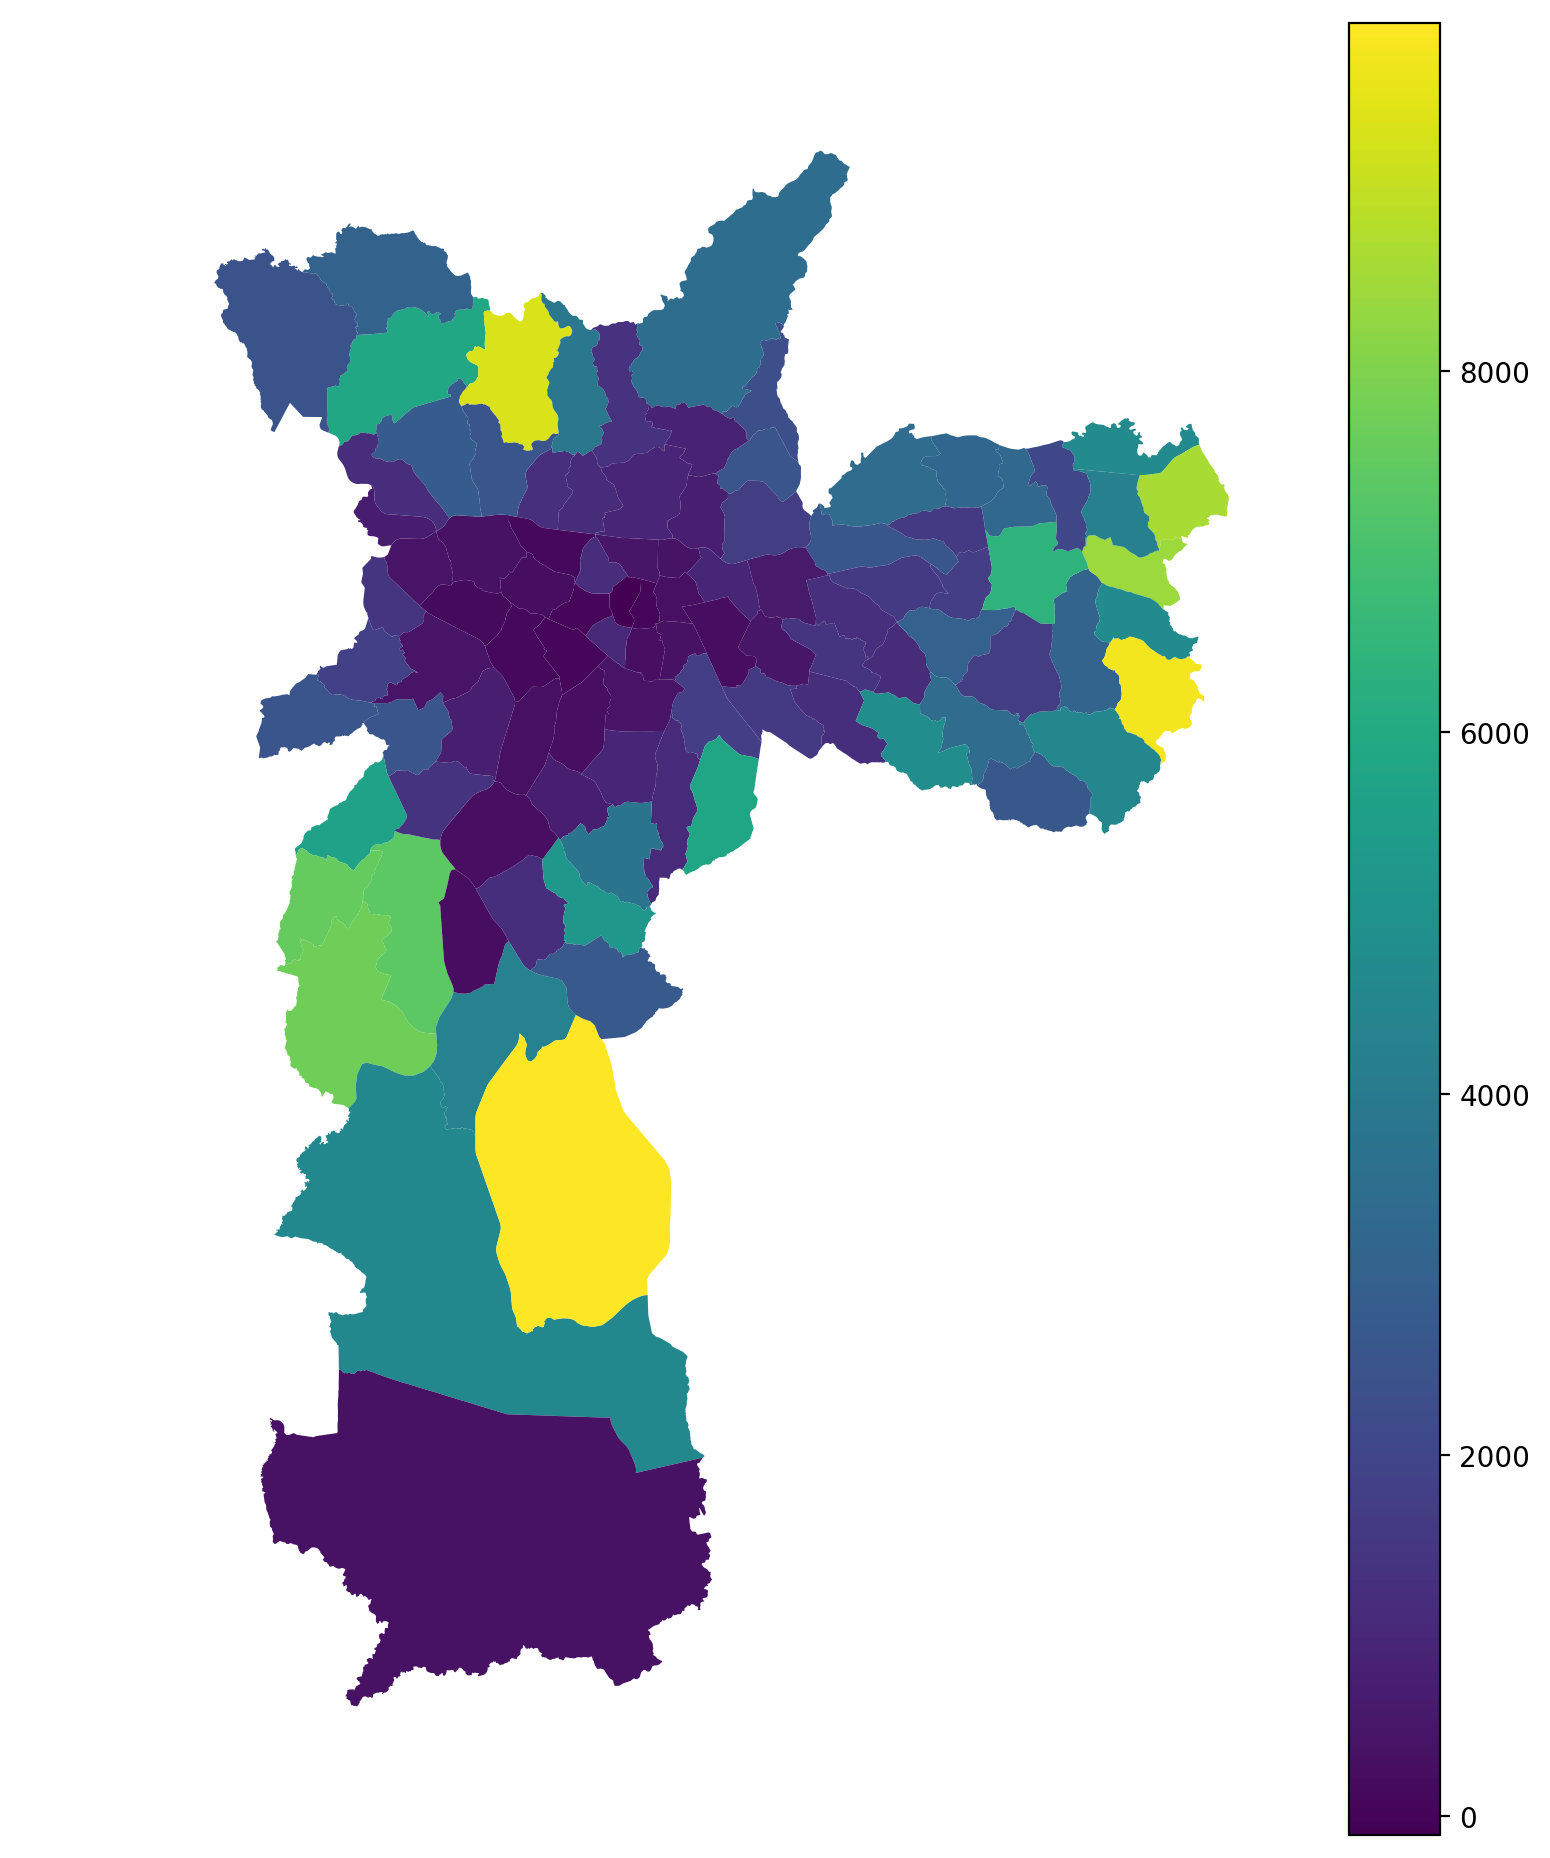
\includegraphics[width=0.475\linewidth]{../Analises/mapas/EV_ABS_NUM_creche.png}
	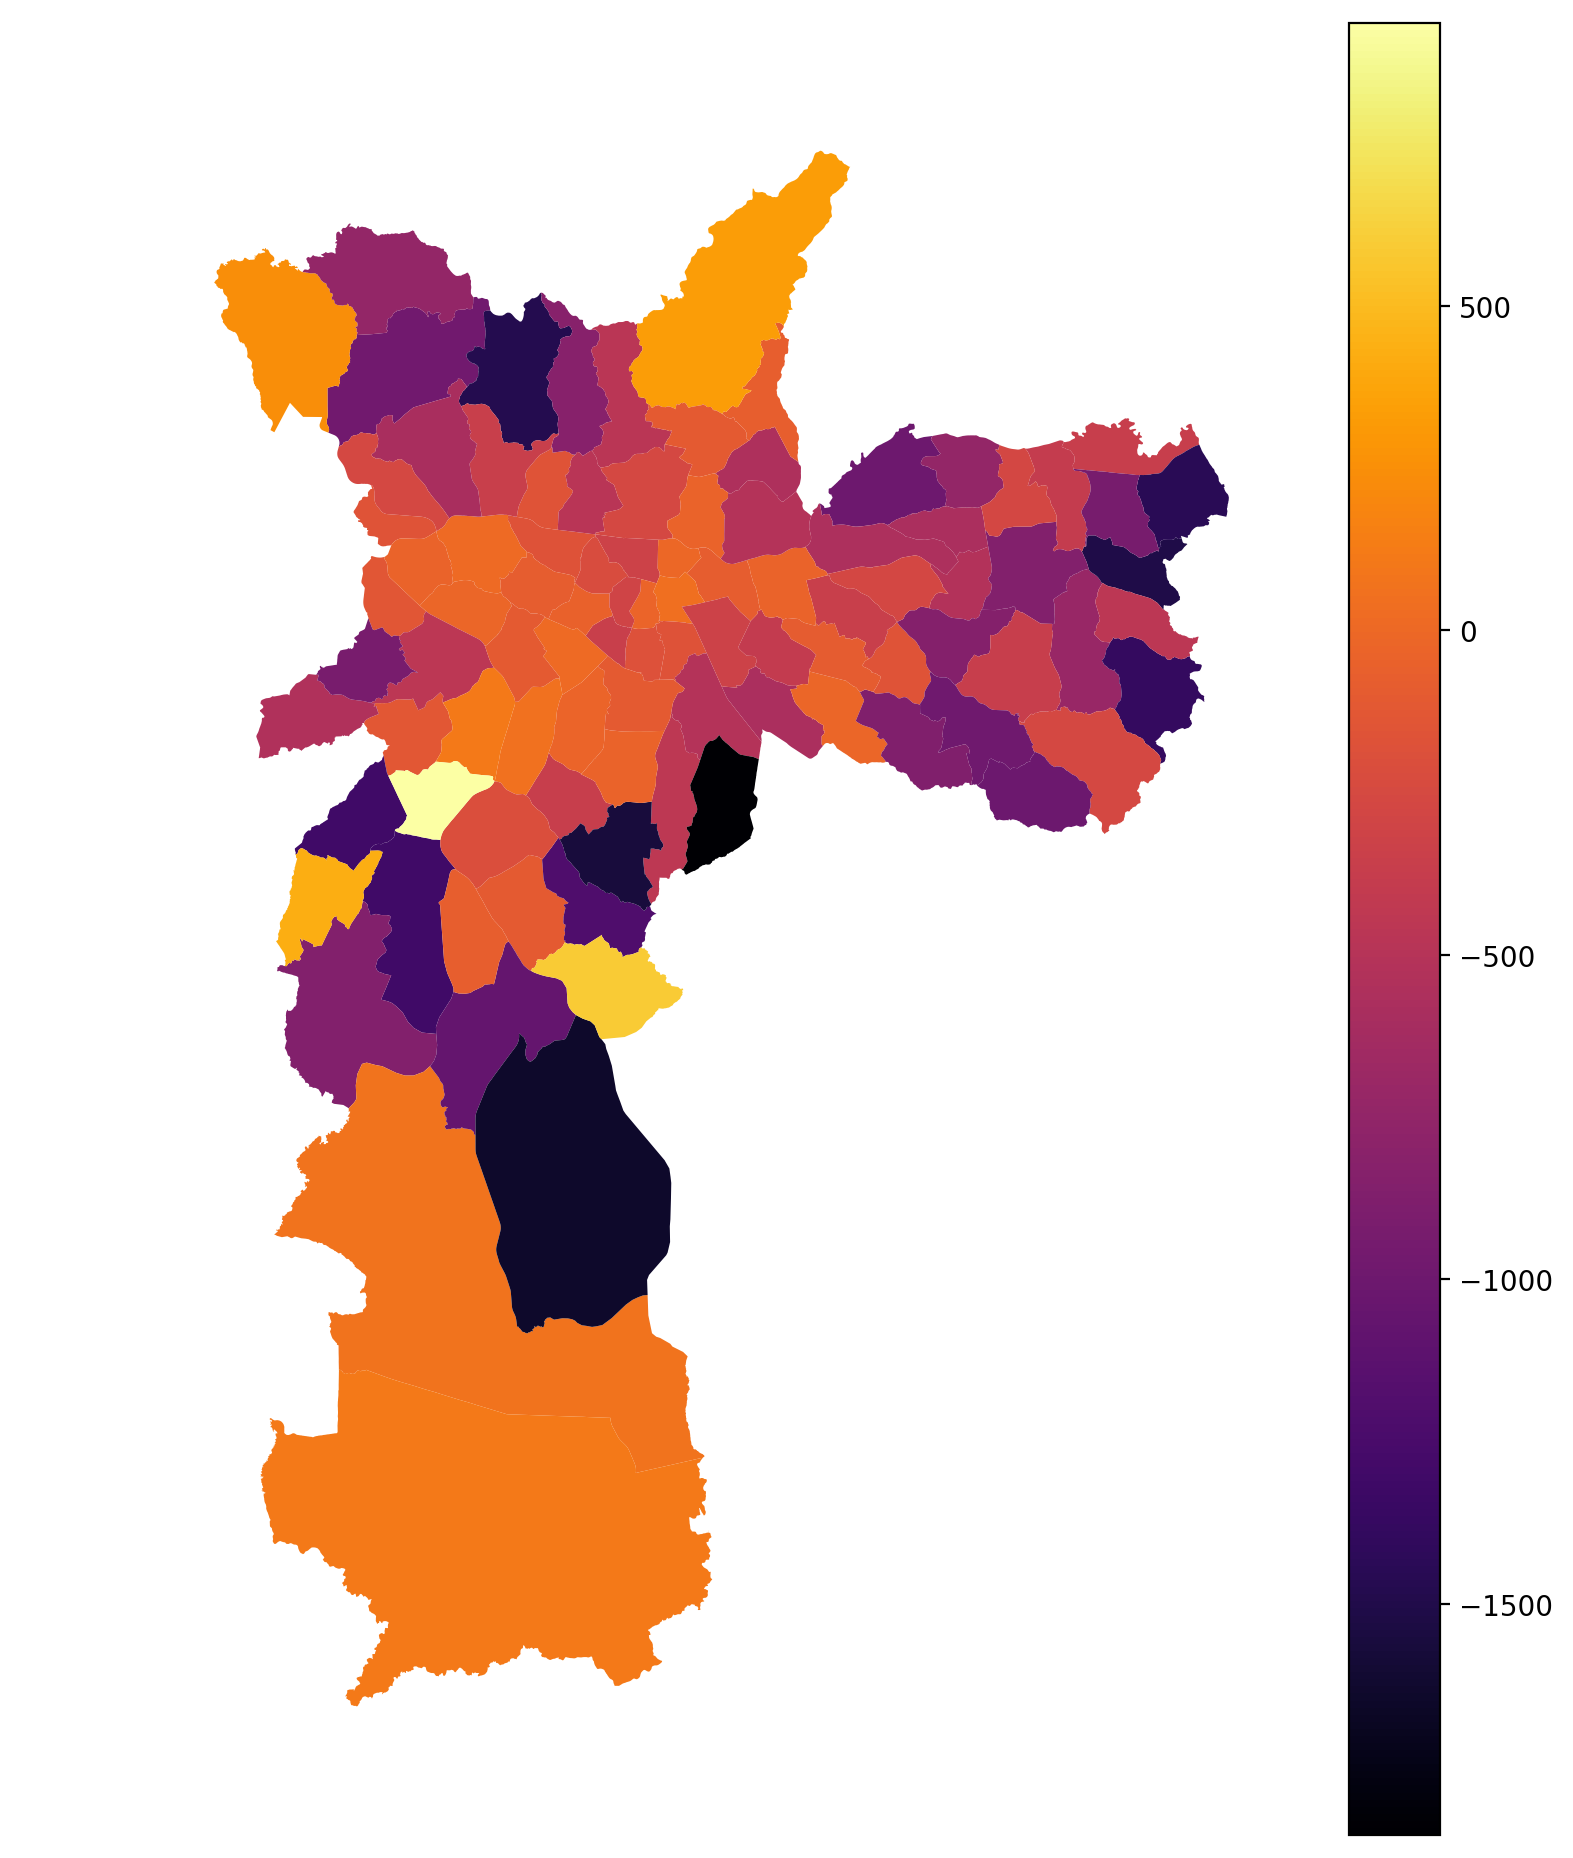
\includegraphics[width=0.49\linewidth]{../Analises/mapas/EV_ABS_NUM_fila.png}
	\caption{Mapas que mostram a evolução geral do número de matrículas entre 06/2006 e 12/2017 e do tamanho da fila, entre 12/2006 e 12/2017, respectivamente.}
	\label{ev:geral}
\end{figure}

